
%\DeclareGraphicsExtensions{.pdf,.png,.JPG}
%\graphicspath{pictures}

\chapter{
Point-Cloud Multi-Contact Planning for Humanoids:\\ Preliminary Results
}

%\author{ \parbox{3 in}{\centering Huibert Kwakernaak*
%         \thanks{*Use the $\backslash$thanks command to put information here}\\
%         Faculty of Electrical Engineering, Mathematics and Computer Science\\
%         University of Twente\\
%         7500 AE Enschede, The Netherlands\\
%         {\tt\small h.kwakernaak@autsubmit.com}}
%         \hspace*{ 0.5 in}
%         \parbox{3 in}{ \centering Pradeep Misra**
%         \thanks{**The footnote marks may be inserted manually}\\
%        Department of Electrical Engineering \\
%         Wright State University\\
%         Dayton, OH 45435, USA\\
%         {\tt\small pmisra@cs.wright.edu}}
%}


%%%%%%%%%%%%%%%%%%%%%%%%%%%%%%%%%%%%%%%%%%%%%%%%%%%%%%%%%%%%%%%%%%%%%%%%%%%%%%%%
\section{abstract}

We present preliminary results in porting our multi-contact non-gaited motion planning framework to operate in real environments where the surroundings are acquired using an embedded camera together with a depth map sensor. %We reconsider each module of our multi-contact planner in view of surrounding models given as 3D point clouds. In this context, two cases are possible: 1) the 3D point cloud is acquired from environments for which we know the objects that compose them; the problem can be turned into point-clouds/model superposition and we still use 3D models of the environment to plan; 2) the 3D point cloud is acquired from environments that we discover (e.g. disaster scenario), in this case we adapt the entire planner to work solely with 3D point clouds. That is, egocentric on-the-fly multi-contact planning, posture generator and collision avoidance based on 3D point clouds.
We consider the robot to have no a priori knowledge of the environment, and propose a scheme to extract the information relevant for planning from an acquired point cloud. This yield the basis of an egocentric on-the-fly multi-contact planner. We then demonstrate its capacity with two simulation scenarios involving an HRP-2 robot in various environment before discussing some issues to be addressed in our quest to achieve a close loop between planning and execution in an environment explored through embedded sensors.


%%%%%%%%%%%%%%%%%%%%%%%%%%%%%%%%%%%%%%%%%%%%%%%%%%%%%%%%%%%%%%%%%%%%%%%%%%%%%%%%
\section{Introduction}

Humanoid robots are expected to move and achieve tasks in ways similar to humans. In cumbersome and unstructured environments, we humans move in a non-gaited acyclic way: we choose appropriate parts of our body to create contacts with the surrounding environment in order to support the motion of the remaining parts while avoiding obstacles. A whole motion is a sequence of contact creations and releases. 

Since we are biped, we mostly use our feet to move. As the environment becomes more difficult to cross, hands may come into play together with feet to help with the motion. Narrow passages may even require other parts of our body (knees, elbows, back...) to make contact in order to support the motion. 

Recently, we have dedicated considerable efforts in proposing a general multi-contact motion planner to solve such cases of non-gaited acyclic planning. Given a humanoid robot, an environment, a start and a final desired postures, our planner generates a sequence of contact stances allowing any part of the humanoid to make contact with any part of the environment to achieve motion towards the goal. A typical experiment with a HRP-2 robot achieving such an acyclic motion is presented in~\cite{escande:iser:2008}, and the planner is thoroughly described in~\cite{escande:ras:2013}. Extensions of this multi-contact planner to multi-agent robots and objects gathering locomotion and manipulation are presented in~\cite{bouyarmane:ar:2012}, and preliminary validations with some DARPA challenge scenarios, such as climbing a ladder, ingress/egress a utility car or crossing through a relatively constrained pathway are presented in~\cite{bouyarmane:humanoids:2012}. In~\cite{escande:ras:2013} and~\cite{bouyarmane:ar:2012}, we describe works in multi-contact that are achieved by other colleagues in robotics.  

All of our previous works, namely the planning scenarios experimented on the HRP-2 humanoid robot, use perfect 3D models of the environment to plan motion. In fact, our previous experiments use model-based, off-line, multi-contact planning. The results are then experimented on the real environment only after a very careful calibration assuming no changes in the object's positions occur during the trials. To achieve dynamic motions that account for whole body motion, we still use off-line planning, see e.g. in~\cite{lengagne:ijrr:2013}. 

Practical implementation and use of our multi-contact planner will not be a plausible option if it cannot be extended to work with data acquired directly from the robot's embedded sensors. Namely, if the environments and composing object models are known, then the robot-environment careful calibration would be ideally done by the robot continuously. In contrast, if the environments and/or composing object models are not known, then the robot must acquire them progressively and build knowledge on which multi-contact planning can still be carried out. This paper examines the possibility to extend our multi-contact planner to work with information acquired by the humanoid embedded visual system, a camera with depth information, providing 3D point cloud data. We assume that we do not have the 3D models of the environment and composing objects. 

Although preliminary, our first trials show promising results. We describe the changes made on our multi-contact planner to work with partial 3D point maps, and present two case studies of successful multi-contact planning simulations on 3D point clouds with the HRP-2 humanoid robot. As a preliminary work, we dedicate a large part of our contribution for discussion.

\section{Background and motivation}

Our multi-contact planning (MCP) is made of several modules. 
\begin{figure}[!htb]
 \centering
 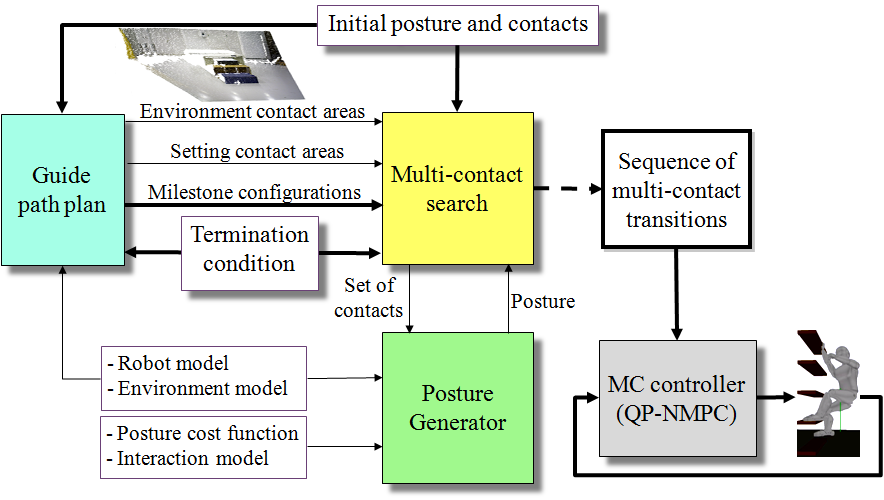
\includegraphics[width=\columnwidth]{papers/RAM2013/pictures/mcp.png}
 \caption{Multi-contact planner architecture.}
 \label{fig:mcp}
\end{figure}
The~\Figref{fig:mcp}{} illustrates the main components and their relation. The core of the planner consists in the multi-contact search and the posture generator. The former incrementally builds a tree of contact sets. The children of a node are obtained by adding or removing exactly one contact to its set. At each iteration of the search, the best leaf, according to a potential field, is expanded this way. The tentative sets of contacts are tested by the posture generator: for a given set of contacts, it attempts to find a configuration of the robot that satisfies these contacts while being statically stable, avoiding collision and staying within the robot's state and torques limits. This is done by automatically writing and solving a non-linear optimization problem. Upon success, the contact set is validated, and a new leaf is created. The goal is written as a set of constraints defining a sub-manifold of the configuration space. A node is the final node if its associated posture generation problem augmented by these constraints remains feasible. By backtracking from this final node to the initial root node, we obtain a sequence of nodes and thus a sequence of contact sets, that can be executed on the robot by a whole-body controller. We developed such a controller based on a quadratic programming (QP) formulation~\cite{bouyarmane:iros:2011}.

The potential field is derived from a crude path, made of a few key postures, that does not take contacts into account. Such a path is either user-defined or can be the output of a first dedicated planner~\cite{bouyarmane:icra:2009}.

The MCP relies largely on the 3D geometric models of the environment and robotic agents. In our previous work~\cite{escande:ras:2013,bouyarmane:ar:2012}, the geometric models are provided by the user. The contact transition for the robot are planned off-line and later executed by the robot assuming exactness of the models and their relative positioning. We aim at extending our MCP to deal directly with real data acquired by the robot. Subsequently, we must deal with two kinds of situations:
\begin{enumerate}
	\item the models of the objects in the environment are known: in this case adapting the MCP consists mainly in dealing with recognition, model superposition and handling uncertainties. In brief, once model superposition is achieved, we can use the 3D model for MCP as in~\cite{escande:ras:2013,bouyarmane:ar:2012}, yet some adjustments are needed.  
	\item the models of the hurdles and the environment are not known (e.g. disaster or outdoor environments, for example related to the Fukushima disaster that inspired the DARPA Robotic Challenge), MCP is to be achieved in an ego-centric way with models built from the robot's embedded sensors. This paper deals with this case and we describe how the MCP is modified to achieve this goal. In a nutshell, we construct planar surfaces from the 3D point clouds data and feed them to the MCP.
\end{enumerate}

In robotics, the use of 3D-based vision for recognition and navigation in environment known or partially unknown has first been used on mobile robots, evolving in flat environment, for example by coupling it with a SLAM system~\cite{whitty:acra:2012}. Another approach consists in extracting the surfaces from the point cloud, and then link them to the known environment or simply consider them as obstacles to be avoided~\cite{poppinga:iros:2008}. Since working on raw point clouds is costly because of the high number of data points, this extraction has also been enhanced~\cite{biswas:icra:2012} in order to be run in real-time. This approach has been recently experimented on a humanoid robot in~\cite{maier:humanoids:2012}, that combines two methods: the surface extraction from a point cloud, and the voxel-based 3D decomposition of the environment~\cite{nakhaei:humanoids:2008}. Still, since the robot only navigates in a flat environment, and does not realize manipulation tasks, the surfaces extracted from the 3D point cloud are down projected to a 2D plan, on which are based the navigation and collision avoidance processes.

The use of humanoid robots allows to navigate in more complex environment, and recently, some work has been done to make a humanoid robot go down a ramp~\cite{lutz:iros:2012} or climb stairs~\cite{osswald:iros:2012}. Yet, those methods use laser-based vision rather than point-cloud-based vision, so as to have a precise analysis of a known environment.

In this work, we aim at enabling a robot to analyze and plan a motion into a 3D environment. Hence, we use the surface extraction of a point cloud to directly have a global picture of the environment and determine the convex planar surfaces that the robot can use at its advantage to progress using the MCP. In our approach to make such an extension, we intentionally seek for technical solutions that minimize changes to be done on our existing MCP software.

\section{Building an understandable environment for our planner}

Our first concern is to build an environment that our multi-contact planner is able to ``understand'' and that can be extracted from a point cloud scene. 
%The simplest kind of entity that our planner would be able to deal with is an oriented rectangular plan surface. Though, it is clear that the real world cannot be precisely described by such things, so we add another level of detail to our world description by using convex polygonal planar surfaces. Therefore, starting from an acquired point cloud, we try to extract a relevant set of such geometrical entities that will be our first description of the surroundings of the robot. 

The simplest entity that our planner would be able to deal with and that could correctly describe the robot's environment is a set of convex polygonal planar surfaces. Therefore, starting from an acquired point cloud, we try to extract a relevant set of such geometrical entities that will be a first description of the surroundings of the robot.

In this section, we present the different steps we follow to create a set of relevant convex polygonal plane surfaces out of an acquired point cloud.
%\begin{itemize}
%\item Acquisition of the point cloud from a RGB and Depth sensor (see section~\ref{subsect:Acquisition})
%\item Filtering the point cloud(see section~\ref{subsect:Filtering})
%\item Plan extraction (see section~\ref{subsect:PlanExtract})
%\item Region growing segmentation(see section~\ref{subsect:region})
%\item Planar projection and hull convex generation (see section~\ref{subsect:PlanProjection})
%\item Re-orientation and transfer to the planner (see section~\ref{subsect:reorient})
%\end{itemize}

The~\Figref{fig:pipeline}{} illustrates the major steps of this point cloud treatment. We use Willow Garage's Point Cloud Library\footnote{\url{http://pointclouds.org/}} (PCL)~\cite{rusu:icra:2011} extensively for processing the point cloud.
\begin{figure*}[!htb]
	  \centering
	    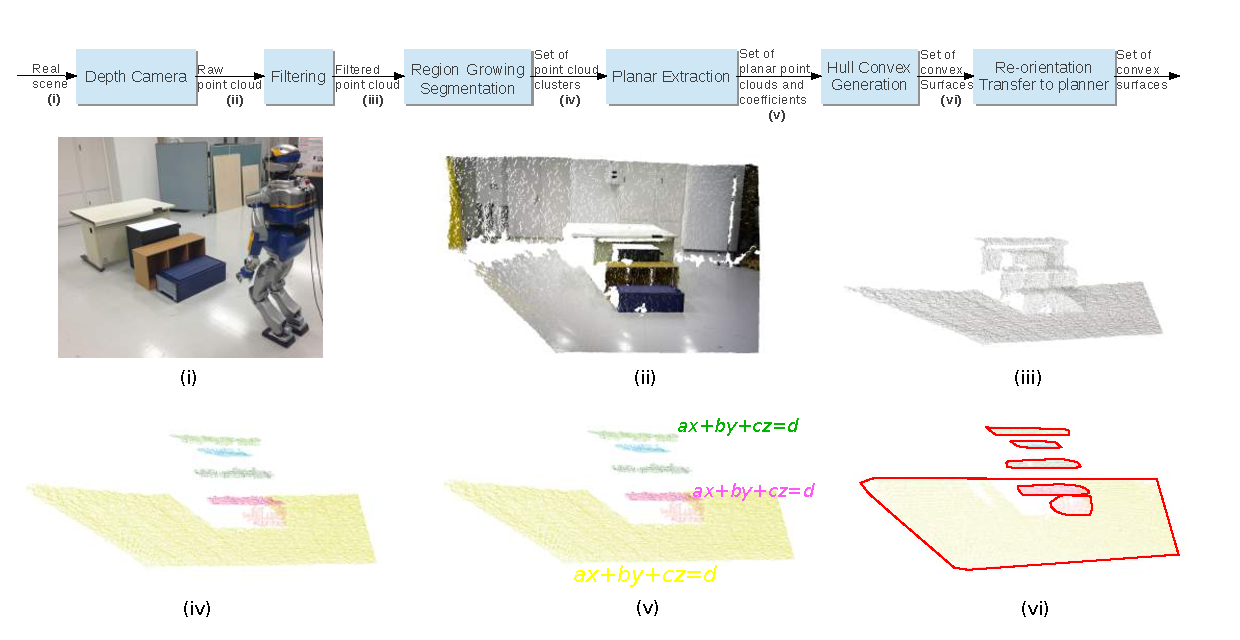
\includegraphics[width=\linewidth]{papers/RAM2013/pictures/complete_pipeline.pdf}
	    \caption{Top: flowchart describing the main elements of our algorithm and the type of data that is passed between them.\newline
	    \hspace*{27pt} Bottom: the data throughout the process, illustrated in the case of our first experiment (see Sec.~\ref{sec:plan1}).}
	    \label{fig:pipeline}
\end{figure*}


\subsection{Acquisition of point cloud from a RGB and depth sensor}
\label{subsect:Acquisition}

For our experiments, we use an Asus Xtion Pro camera, that provides a $640 \times 480$ pixel depth image, and the OpenNI Grabber. The obtained point cloud representing our scene contains points defined by their space coordinates and colors, and will be the entry of our point cloud treatment algorithm. We do not use the color information for now except for display purpose. It may however be useful in the future in matching object models with sensor data and to perform color-based region growing algorithms.

%\subsection{Parsing the .pcd file}
%
%This "initialization" step of our algorithm is staightforward; PCL implements some method to create a PointCloud object's
%instance directly out of a .pcd file.

\subsection{Filtering}
\label{subsect:Filtering}

In order to reduce the computation time and improve the efficiency of our point cloud treatment algorithm, it is necessary to reduce the overall size of the data set. We first remove all points further than 5 meters from the camera: such points are not reliable enough and thus a potential source of error for the following steps.
%We know that the data extracted from the Asus Xtion live camera are reliable only for points that are less than 5 meters away from it. Therefore, we eliminate all the 
%points that are further than that, since they would only be a source of error and wouldn't carry any valuable information.

We then downsample the cloud, since it is excessively dense for our purpose. To do so, we use a voxelized grid approach (using the {\tt pcl::VoxelGrid} class): we create a 3D voxel grid over the input point cloud data. Each voxel represents a group of points that are close enough from each other to be represented by a single point that would be their centroid. The centroid is chosen instead of the center of the voxel because it represents the real environment more accurately. Another advantage of this method is that the filter can easily be parametrized by choosing the size of the voxels. Those two steps allow us to greatly reduce the number of points in the data set. Typically, in our experiments, this divides the number of points by a factor 5 to 6.

\subsection{Region growing segmentation}
\label{subsect:region}

In order to divide a global point cloud scene into several sets of points that belong to the same flat area, we use a region growing algorithm~\cite{poppinga:iros:2008} (implemented in {\tt pcl::RegionGrowing} class). Its purpose is to merge the neighboring points that are close enough in terms of smoothness constraint. The output of this algorithm is a set of clusters representing sets of points that are considered to be a part of the same plane surface. This method is based on the comparison of the angles between the points' normals. 
%\note{\sout{This algorithm fits perfectly our needs, because it provides us with a list of sub-clouds (clusters), and each of those represents a flat area of the scene.}}
It is used right before the planar extraction algorithm in order to obtain an accurate list of points and plane models they represent. 

\subsection{Planar extraction}
\label{subsect:PlanExtract}

We use a plane segmentation to extract and group all the points that support a same plane model. Thus, we obtain a set of distinct point clouds. Indeed, this method finds the plane model that can carry the biggest set of points without regard for their proximity to each other. Then this first set of points is extracted from the initial point cloud and the algorithm can be applied to the remaining cloud recursively until the remaining cloud is small enough (in terms of number of points). For this purpose, we use the {\tt pcl::SACSegmentation} class.

This process works better on mostly flat point clouds (composed of a small number of large plane surfaces). Indeed, if it is applied to a point cloud that represents some stairs, instead of finding a set of points and a plane model for each step, it will most likely find a set of points and a plane model that represent the average slope of the stairs, and the reason for that is that the criteria of choice of a plane model is the greater number of points it bears, no importance is given to the proximity between the points of a planar set. That is why we apply the region growing algorithm~\ref{subsect:region}, that provides a list of clusters that represent the flat surfaces of the scene, before applying the planar extraction process on each of those clusters. 
It then computes a correct set of points and a plane model per region cluster.

\subsection{Planar projection and hull convex generation}
\label{subsect:PlanProjection}

The exact knowledge of all the data points contained in the plane model of a flat area is not necessary for our planning; we can reduce the point cloud to its convex hull without loss of information (except if the surface is concave, but this issue will be tackled in future works). In order to obtain the convex hull of each set of points, we first project every point of the set on its plane model ({\tt pcl::ProjectInliers} class) and then compute the 2D convex hull of the projected set of points ({\tt pcl::ConvexHull} class). After this step, each plane surface of the scene is represented by a frame composed of 3 vectors that are respectively a tangent, bi-tangent and normal vector of the plane model, an origin point that is the barycentre of the set of points and a small set of points that define its convex hull (the points' coordinates being calculated in the referential defined by the frame and the origin of the surface in order to make further calculations easier).

\subsection{Re-orientation and transfer to the planner}
\label{subsect:reorient}

Before sending the previously computed data to the planner, it is necessary to take into account the initial orientation of the camera. Indeed, if the camera was not aiming in a perfectly horizontal direction, then the entire point cloud would be misoriented. Therefore, it is necessary to re-orientate the surfaces before sending them to the planner. To do so, we simply apply a rotation matrix (that is computed from the initial camera orientation) to each of our data set's frame and origin to settle that problem. From there, the transfer of the surfaces to the planner can be done without any specific issue.

Re-orientation is done as a last step for the sake of performance: obviously we need to re-orient only a few frames, compared to an early re-orientation of the point cloud that would require to apply a transformation on thousands of points.

\section{Planning on point clouds}
\subsection{Convex surfaces inclusions}
We adjusted slightly our planner and posture generator to handle contacts between convex polygonal plane surfaces. The main modification made in the posture generator deals with properly writing the constraints that enforce the inclusion of one surface into another one. In our previous implementation, contacts are searched between rectangular patches attached to the robot body or the environment. Now any polygonal convex-shaped patch can be checked for inclusion in another; that is to say, the vertices of a convex 2D polygon are indexed counter-clockwise around its carrying plane surface's normal vector. A point that is inside the polygon is on the left side of all its edges. On the opposite, a point that is outside of the polygon will be on the right side of at least one of the polygon's edges. The following is the algorithm we use for the constraint generation:
\begin {algorithm}
\caption{Surface inclusion constraints for $S_i \subset S_j$}
\label{alg1}
\begin{algorithmic}
\STATE {Let $S_i$ and $S_j$ be two coplanar plane surfaces}
\STATE {$S_i = {p_0, p_1, \ldots, p_n}$ and $S_j = {q_0, q_1, \ldots, q_m}$}
\STATE {$\vec{N}$ is $S_i$'s normal vector}
\FOR{$k = 0 \to n$}
\FOR{$l = 0 \to m$}
\STATE { Constraint $: \left[\overrightarrow{q_lp_k}\times\overrightarrow{q_lq_{l+1}}\right].\vec{N} \leq 0$}
\ENDFOR
\ENDFOR
\end{algorithmic}
\label{algo:constraints}
\end{algorithm}

For a couple of coplanar surfaces $S_i$, $S_j$ respectively represented by $n$ and $m$ points, we create $n \times m$ constraints to ensure that the former is included in the latter one.

Once the surfaces are defined, it is possible to choose which ones are suitable for the robot to make contact with. Although it is not a mandatory step, it allows to reduce the exploration during the planning phase by removing undesired or inappropriate pairs of robot/environment surfaces. For the time being, this is determined by heuristics that are defined depending on the situation. For example, if we want the robot to walk on various surfaces, only surfaces that have a normal vector closely aligned with the gravity field would be selected as potential candidates (so as to eliminate the walls and other surfaces on which the robot cannot walk). Similarly, only surfaces located at a certain height can be considered for hand contact, etc.

\subsection{Collision detection}

In order to generate a feasible plan, we need to ensure that the robot avoids collisions with its environment and with itself. To do so, we consider each surface generated by our point cloud treatment algorithm as a thin 3D body. Basically, we extrude each surface by few centimetres in the direction opposite to its normal (provided that this normal is pointing toward the outside of the real body) and create a convex hull surface using {\tt QHull}~\cite{qhull:ACM:1996}. The collision avoidance is then computed by using the {\tt GJK} algorithm implemented efficiently for several convex shapes in~\cite{benallegue:icra:2009}.


\section{Results} 

In order to illustrate our method, we present two experiments in which the HRP-2 robot is asked to move $2$m forward. In both scenarios, this results in climbing on a table (The first one is $0.71$m-high and the second one is $0.53$m-high) with the help of various surrounding objects. The knowledge about the environment and surrounding objects is obtained from a point cloud captured by an ASUS Pro Xtion camera in one single shot. The camera was placed at the height of the robot's head, see~\Figref{fig:pipeline}{}.

All the computations of the following experiments are performed on a single thread of an Intel(R) Core(TM) i7-3840QM CPU at 2.80GHz, with 16Go of RAM.

\subsection{Plan 1: irregular stairs}
\label{sec:plan1}


In this first experiment, the robot has to walk up some irregular stairs made of several random pieces of furniture to reach its goal. The filtered point cloud contained 60286 points, that were split into 6 plane surfaces. The whole cloud processing was done in $2.7$ s. The planner computations generates a path of 11 nodes, some of which are depicted in~\Figref{fig:table-climbing-simulation-stair}{}. We notice that the robot climbs the stairs one by one without ever putting its two feet on the same step and without any noticeable problem.
In total, 23 nodes were generated and the planning time was $98.4$ s.

\begin{figure*}[!htb]
	\centering
	\renewcommand{\arraystretch}{0.2}
	\begin{tabular}{l c r}
	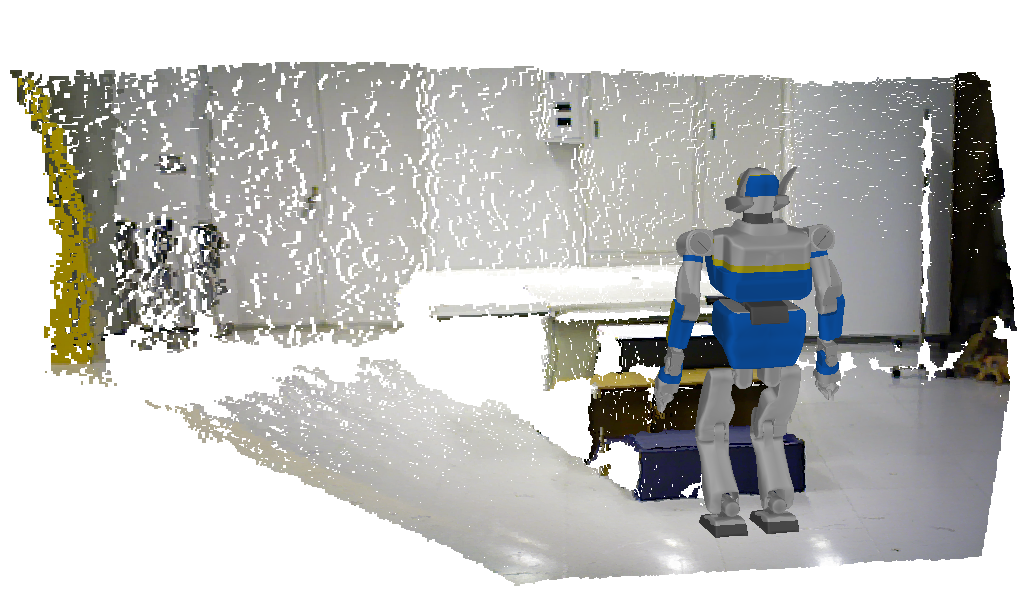
\includegraphics[width=.308\linewidth]{papers/RAM2013/pictures/Simu11Step0.png}&
	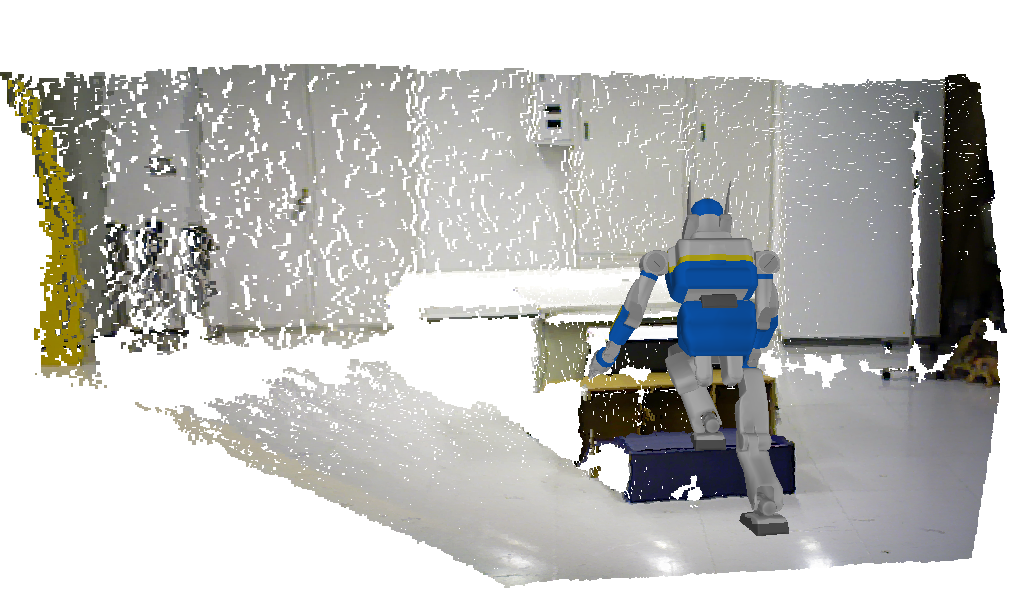
\includegraphics[width=.308\linewidth]{papers/RAM2013/pictures/Simu11Step3.png}&
	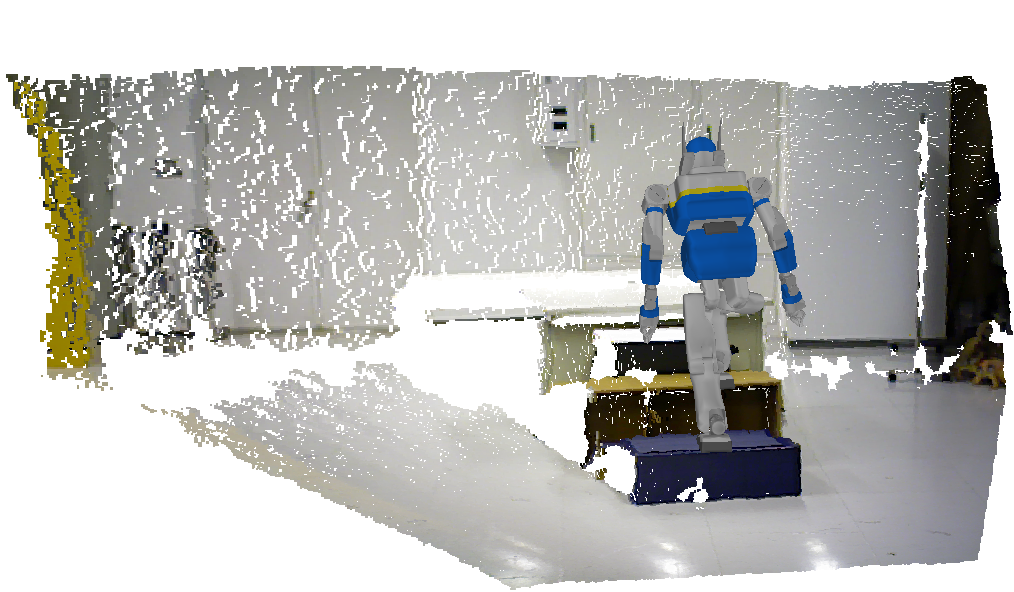
\includegraphics[width=.308\linewidth]{papers/RAM2013/pictures/Simu11Step5.png}\\
	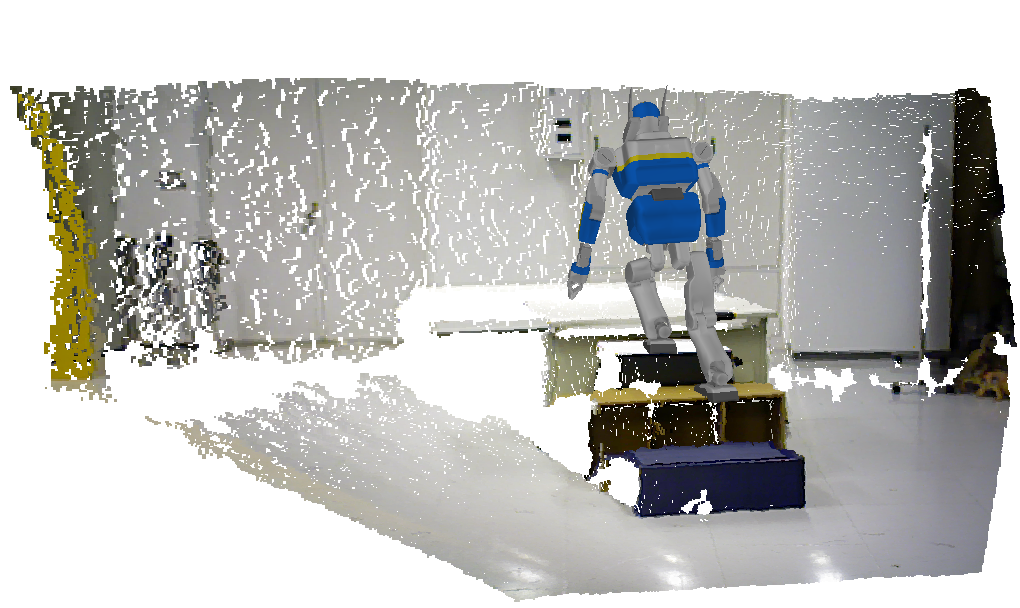
\includegraphics[width=.308\linewidth]{papers/RAM2013/pictures/Simu11Step7.png}&
	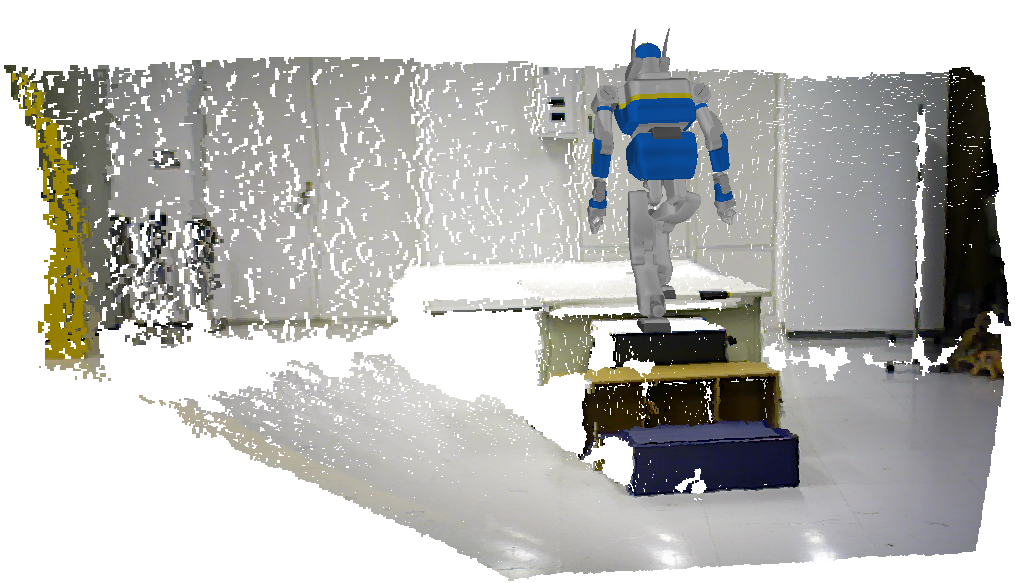
\includegraphics[width=.308\linewidth]{papers/RAM2013/pictures/Simu11Step9.png}&
	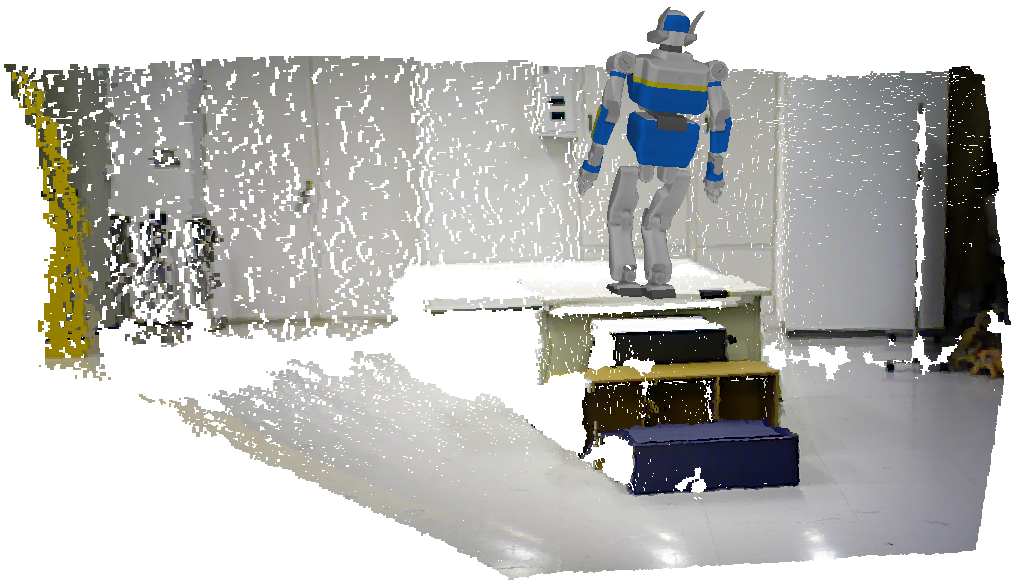
\includegraphics[width=.308\linewidth]{papers/RAM2013/pictures/Simu11Step10.png}\\
	\end{tabular}
	\caption{Table climbing simulation using irregular stairs. Of the 11 nodes of the path, we depicted the nodes 1, 4, 6, 8, 10 and 11.}
	\label{fig:table-climbing-simulation-stair}
\end{figure*}


\subsection{Plan 2: helping motion with the hand}
This second experiment was designed to showcase a more complex plan involving the use of the HRP-2 upper limbs. In this experiment, the filtered point cloud contained 66907 points, from which 11 surfaces were extracted. The whole cloud processing was done in $2.7$ s. The planner computation generates a path of 19 nodes, some of which are depicted in~\Figref{fig:crapahut-simulation}{}. To climb on the table, the robot uses its left arm and walks on an inclined slope before climbing a step at the end of the slope, once again, with the help of its left arm as support. In total, 40 nodes were generated and the planning time was $122.3$ s.

\begin{figure*}[!htb]
	\centering
	\renewcommand{\arraystretch}{0.2}
	\begin{tabular}{l c r}
		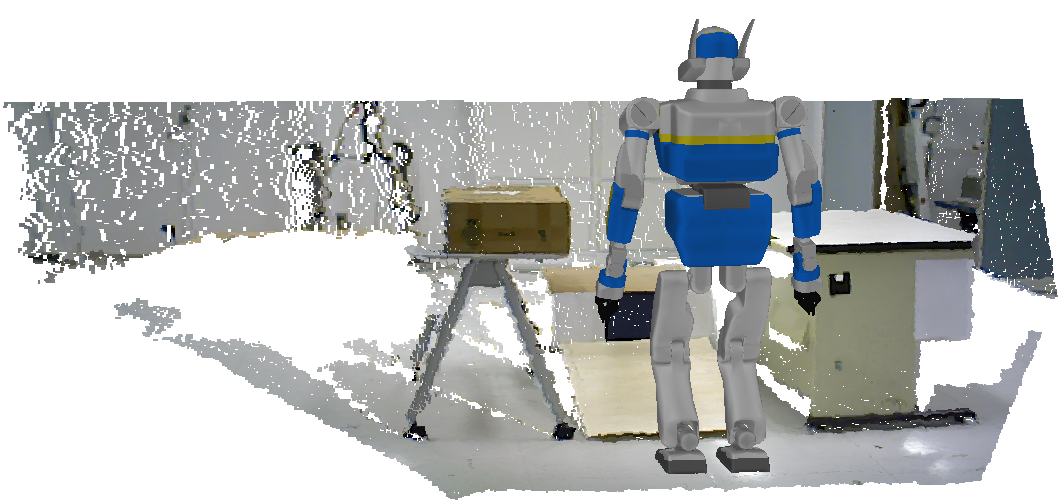
\includegraphics[width=.308\linewidth]{papers/RAM2013/pictures/Simu9Step0.png}&
		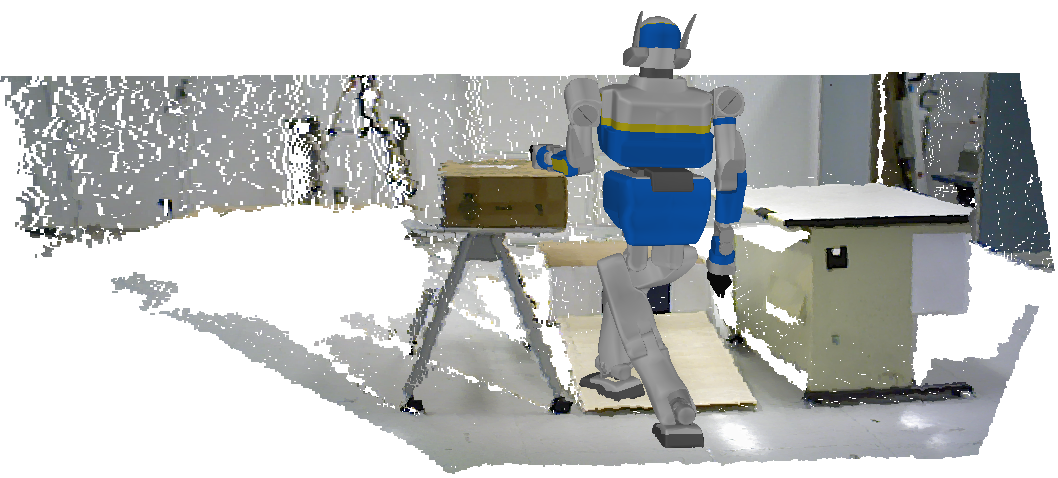
\includegraphics[width=.308\linewidth]{papers/RAM2013/pictures/Simu9Step6.png}&
		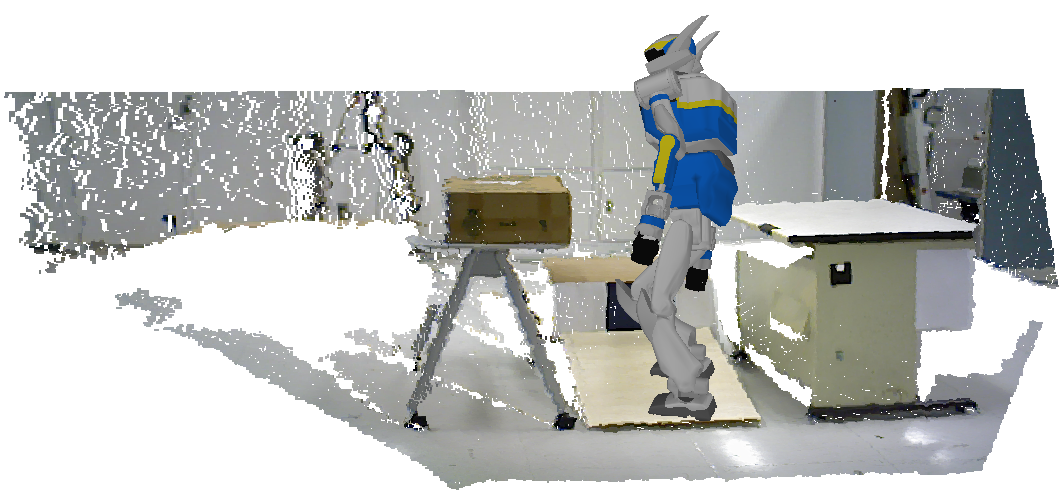
\includegraphics[width=.308\linewidth]{papers/RAM2013/pictures/Simu9Step11.png}\\
		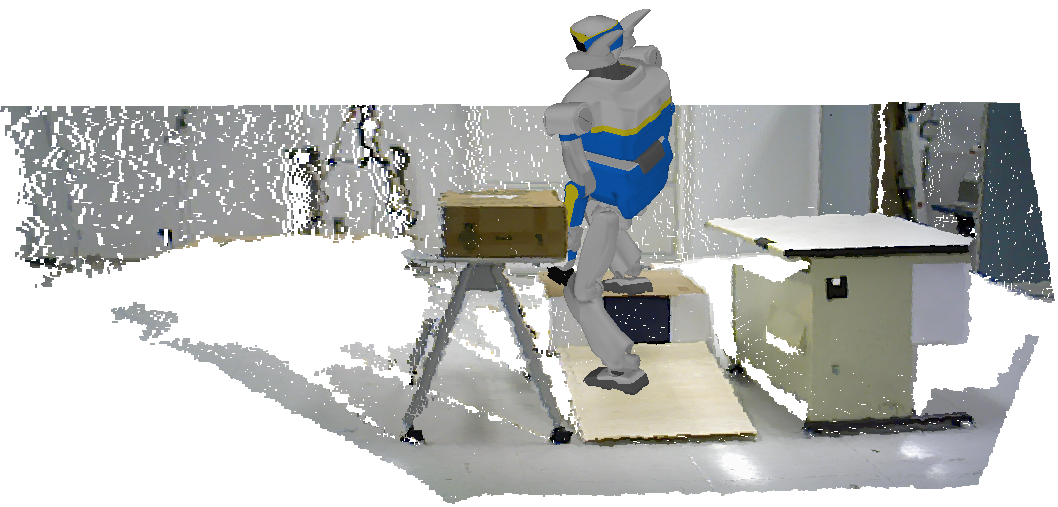
\includegraphics[width=.308\linewidth]{papers/RAM2013/pictures/Simu9Step14.png}&
		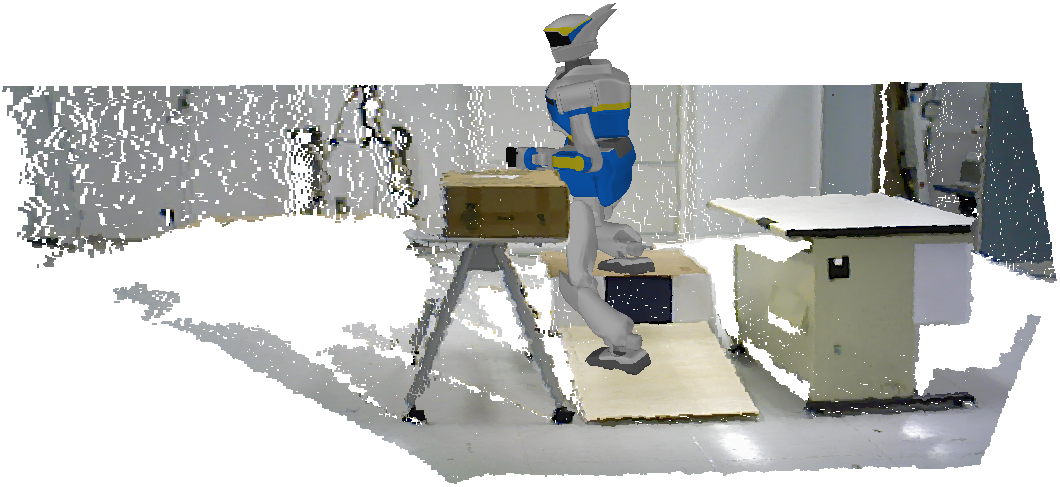
\includegraphics[width=.308\linewidth]{papers/RAM2013/pictures/Simu9Step16.png}&
		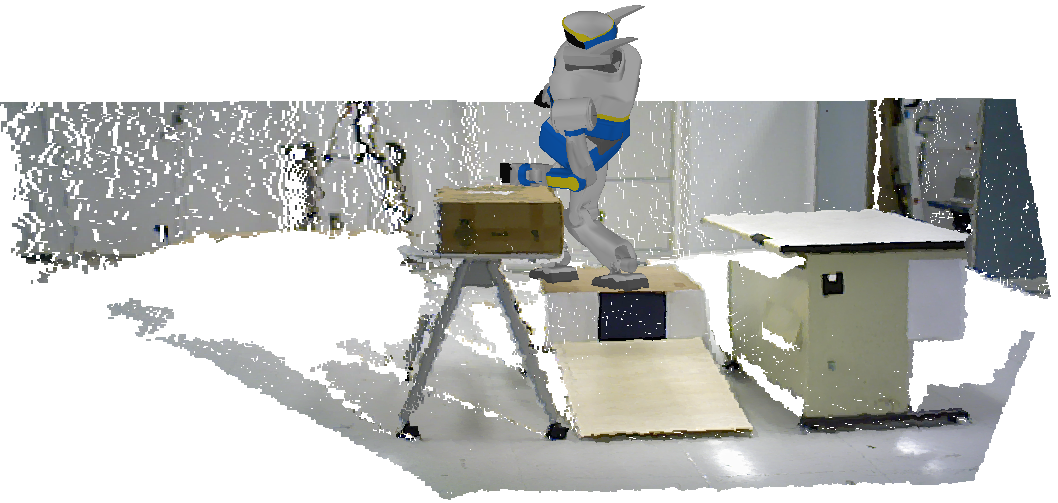
\includegraphics[width=.308\linewidth]{papers/RAM2013/pictures/Simu9Step17.png}\\
	\end{tabular}
	\caption{Slope and step climbing simulation. Of the 19 nodes of the path, we depicted the nodes 1, 7, 12, 15, 17 and 18.}
	\label{fig:crapahut-simulation}	
\end{figure*}


\section{Discussion}
This work is a first step toward a fully sensory-perception-based multi-contact planner. It raises several interesting questions on the way to adapt our MCP. 

One advantage of our approach is to avoid having to precisely position the robot in the environment prior to the plan execution. Yet, for now the positioning is done once and for all with the acquisition of the point cloud, before planning. When executing the plan, the robot might still deviate from it, for example a support might move, or a foot might contact a few centimetres away from where it was planned to, or the support might not be at its expected position because of measurement errors in the acquired point cloud. We thus need to close the loop between the planning and its execution. To do so, we need robust detection of discrepancies to be made by the robot. This can be achieved by combining point-cloud-based SLAM with contact sensing. Once the robot has acquired knowledge of its deviation or of the position error of the support, it has to adapt to it. This adaptation should not be time-consuming so as to not interrupt the execution for too long. A slight deviation can be recovered by simply positioning with care the next contacts and the closed-loop multi-contact controller shall work on guarded-motions basis. However, a bigger deviation might make the next contact stances infeasible. In this later case, re-planning the next contacts is necessary to go back to the plan. How many contacts have to be re-planned depends on the context. In difficult situations, changes in contacts might cascade up to requiring an entire re-planning. Recognizing the situation should be the task of a local planner that re-plans as few steps as possible. In case too much contacts must be reprocessed, the re-planning phase can be stopped before it ends and resumed at the next step.

This partial planning approach can also be seen in the context of semi-autonomous motion: an operator gives the overall direction with, for example, a joystick, and the planner reactively finds a sequence of a few contact sets to move as closely as possible in this desired direction. The operator is thus in charge of preventing the robot from getting stuck while the planner only concentrates on finding the correct contacts over a short time window.

Another question stems from the partial knowledge of the environment: it is not possible to give a guide path as we used to do with the 3D models. This guide path will necessarily be very crude, either a line to a desired position, or a plan in a known environment before it was changed (for example in the case of a disaster in a plant). The planning must then be driven also by the need of getting information about the environment, for example reaching a viewpoint allowing to see parts of the environment that were hidden before, filling empty spaces and possibly adding new supports on-the-fly. Planning is then only partial since necessary part of the environment might be unknown. 

Later on, the discovery of the environment might be improved by the use of other sensors. One can then imagine having the robot test for a contact to ensure a given surface is fit for support or that it is precisely at the position measured by vision. If the surface is not, this is another kind of discrepancy in the plan than needs to be handled by re-planning. 

\section{Conclusion}
We present preliminary results in extending our previous work in multi-contact planning to operate directly on environment that is built on-the-fly from a robot's embedded sensors. This first study makes use of depth camera and implemented modules from the PCL which extract planar surfaces that are fed to our MCP. We intentionally seek for technical implementations that minimize the changes on our existing MCP software and illustrate successful plans generated on the basis of 3D point clouds solely. 

The simulation results revealed that indeed our MCP does not require major adjustments to handle egocentric sensory data. Of course, this does not mean that we are fully satisfied since our results also suggest additional future work. 

First, although we choose to treat the case of not having 3D models, we believe that the implementation of an MCP with knowledge of the 3D model is necessary. For example, even in a disaster situations as in Fukushima nuclear power plants, the inside exploration videos available show that many objects kept their shape and were not totally destroyed (e.g. door, stairs, ladders, etc.). So having their model would then still permit our MCP to rely on 3D models to plan contacts for motion. PCL provides only partial information, it is then necessary to drive the planner by the mission objective and also a perceptual one (e.g. SLAM). Of course, our ultimate future plan is to handle uncertainties, control and planning recovery of discrepancies when they occur.
